\documentclass[tikz,border=4pt]{standalone}
\usepackage{tikz}
\usetikzlibrary{shapes.geometric,arrows.meta,positioning}

\begin{document}
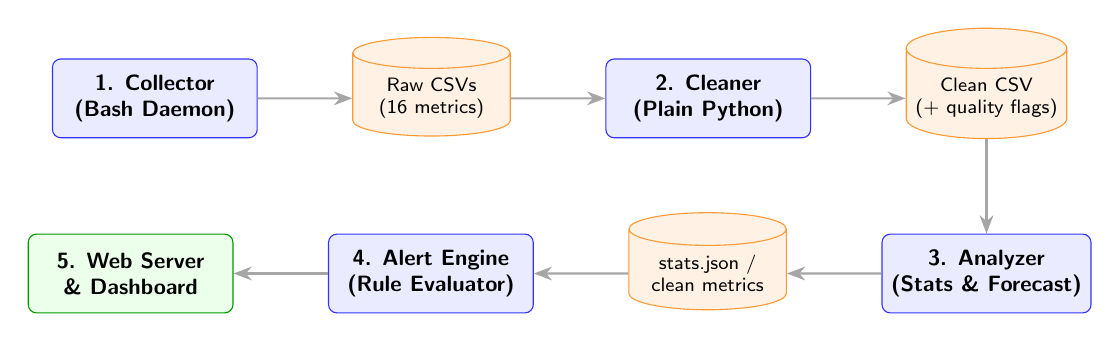
\begin{tikzpicture}[
    node distance=0.9cm and 1.2cm,
    stage/.style={rectangle, draw=blue!80, fill=blue!8, rounded corners=3pt, minimum width=2.6cm, minimum height=1.0cm, align=center, font=\sffamily\footnotesize\bfseries},
    data/.style={cylinder, shape border rotate=90, aspect=0.25, draw=orange!80, fill=orange!10, minimum width=2.0cm, minimum height=0.8cm, align=center, font=\sffamily\scriptsize},
    ui/.style={rectangle, draw=green!60!black, fill=green!8, rounded corners=3pt, minimum width=2.6cm, minimum height=1.0cm, align=center, font=\sffamily\footnotesize\bfseries},
    link/.style={->, >=Stealth, thick, draw=gray!70}
]

\node[stage] (coll) {1. Collector\\(Bash Daemon)};
\node[data, right=of coll] (raw) {Raw CSVs\\(16 metrics)};
\node[stage, right=of raw] (clean) {2. Cleaner\\(Plain Python)};
\node[data, right=of clean] (cdata) {Clean CSV\\(+ quality flags)};
\node[stage, below=1.2cm of cdata] (analy) {3. Analyzer\\(Stats \& Forecast)};
\node[data, left=of analy] (stats) {stats.json /\\clean metrics};
\node[stage, left=of stats] (alerts) {4. Alert Engine\\(Rule Evaluator)};
\node[ui, left=of alerts] (web) {5. Web Server\\\& Dashboard};

\draw[link] (coll) -- (raw);
\draw[link] (raw) -- (clean);
\draw[link] (clean) -- (cdata);
\draw[link] (cdata) -- (analy);
\draw[link] (analy) -- (stats);
\draw[link] (stats) -- (alerts);
\draw[link] (alerts) -- (web);

\end{tikzpicture}
\end{document}
